%%%%%%%%%%%%%%%%%%%%%%%%%%%%%%%%%%%%%%%%%%%%%%%%%%%%%%%%%%%%%%%%%%%%%%%%%%%%%%%%
% FYP-I PROPOSAL DOCUMENT FOR COMSATS UNIVERSITY
% Generated by Google's AI Assistant
% Instructions:
% 1. Upload your university logo and name it 'logo.png'
% 2. Upload your system block diagram and name it 'block_diagram.png'
% 3. Click "Recompile" to generate the PDF.
%%%%%%%%%%%%%%%%%%%%%%%%%%%%%%%%%%%%%%%%%%%%%%%%%%%%%%%%%%%%%%%%%%%%%%%%%%%%%%%%

\documentclass[12pt, a4paper]{article}

% PACKAGES FOR FORMATTING AND IMAGES
\usepackage[margin=1in]{geometry} % Sets page margins to 1 inch
\usepackage{graphicx}             % To include images
\usepackage{helvet}               % Uses Helvetica-like font for a modern look
\usepackage{tabularx}             % For better tables
\usepackage{array}                % For advanced table column formatting
\usepackage{amsfonts}             % Math fonts
\usepackage{amsmath}              % Math environments
\usepackage{titlesec}             % To customize section titles
\usepackage{hyperref}             % For clickable links in the PDF

% --- DOCUMENT FORMATTING ---

% Set the default font to sans-serif (like in the template)
\renewcommand{\familydefault}{\sfdefault}

% Set line spacing to 1.5 for readability
\linespread{1.5}

% Customize section headings to be large and bold
\titleformat{\section}{\Large\bfseries}{\thesection.}{1em}{}
\titleformat{\subsection}{\large\bfseries}{\thesubsection.}{1em}{}

% Hyperlink setup for a clean look
\hypersetup{
    colorlinks=true,
    linkcolor=black,
    urlcolor=blue,
    citecolor=black,
}

% --- DOCUMENT START ---
\begin{document}

% --- TITLE PAGE ---
\begin{titlepage}
    \centering
    \vspace*{0.5cm}
    
    % University Logo and Header
    
\includegraphics[width=0.2\textwidth]{logo.png}\par
    \vspace{0.5cm}
    {\Large\bfseries COMSATS University Islamabad, Lahore Campus}\par
    {\large\bfseries Department of Computer Engineering}\par
    \rule{\textwidth}{1.5pt}
    \vspace{1.5cm}
    
    {\huge\bfseries FYP-I Project Proposal}\par
    \vspace{1.5cm}
    
    % --- PROJECT DETAILS BOXES ---
    \begin{flushleft}
    % Project Title Box
    \noindent\fbox{%
        \parbox{\dimexpr\textwidth-2\fboxsep-2\fboxrule}{%
            \textbf{Project Title} \par
            \vspace{0.5cm}
            Two-Layer Contactless Physical Authentication System: Combining Facial \& Voice Recognition
            \vspace{0.5cm}
        }%
    }
    
    \vspace{1cm}
    
    % Project Supervisor Box
    \noindent\fbox{%
        \parbox{\dimexpr\textwidth-2\fboxsep-2\fboxrule}{%
            \textbf{Project Supervisor} \par
            \vspace{0.5cm}
            Dr. Zaid Ahmad
            \vspace{0.5cm}
        }%
    }
    \end{flushleft}
    
    \vspace{1cm}
    
    % --- GROUP MEMBERS TABLE ---
    \noindent
    \begin{tabular}{| >{\bfseries}l | m{4cm} | m{4cm} | m{5cm} |}
        \hline
        \multicolumn{4}{|l|}{\bfseries Group Members} \\
        \hline
         & \textbf{Name} & \textbf{Reg. ID} & \textbf{Email Address} \\
        \hline
        \textbf{1} & Abdullah Laeeq & CIIT/FA22-BCE-026/LHR & fa22-bce-026@cuilahore.edu.pk \\
        \hline
        \textbf{2} & Ali Hamza & CIIT/FA22-BCE-071/LHR & fa22-bce-071@cuilahore.edu.pk \\
        \hline
        \textbf{3} & Muhammad Faizan Shurjeel & CIIT/FA22-BCE-086/LHR & fa22-bce-086@cuilahore.edu.pk \\
        \hline
    \end{tabular}
    
    \vspace{1cm}
    
    % Comments Box
    \noindent\fbox{%
        \parbox[t][6cm][t]{\dimexpr\textwidth-2\fboxsep-2\fboxrule}{%
            \textbf{Comments about the Group and the Project Scope:} \par \vspace{0.3cm}
            This project aims to develop a robust, two-factor biometric authentication system as a proof-of-concept. The scope includes researching state-of-the-art AI models, developing independent facial and voice recognition pipelines, integrating them into a cohesive system, and implementing foundational anti-spoofing measures. The final goal is to create a Minimum Viable Product (MVP) suitable for deployment on low-cost embedded hardware, demonstrating a practical and innovative solution to modern security challenges.
        }%
    }
    
    \vfill % Pushes the rest to the bottom
    
    % --- FOOTER ---
    {\bfseries Department of Computer Engineering \par
    COMSATS University Islamabad \par
    LAHORE Campus – PAKISTAN}
    
\end{titlepage}

% --- MAIN DOCUMENT CONTENT ---

\newpage
\tableofcontents
\newpage

% --- SECTION 1: ABSTRACT ---
\section{Abstract}

Traditional authentication methods, such as passwords, PINs, and physical tokens, are increasingly proving to be insufficient in the face of modern security threats like phishing and data breaches. Furthermore, the global emphasis on hygiene following the COVID-19 pandemic has highlighted the risks associated with contact-based biometric systems like fingerprint scanners. This project addresses these security and hygiene gaps by proposing a Two-Layer Contactless Physical Authentication System. The system leverages the unique biometric markers of an individual's face and voice to provide a highly secure, convenient, and touch-free method of identity verification. The primary goal is to create a seamless user experience applicable to a wide range of scenarios, including physical access control for buildings, attendance tracking in educational and corporate settings, and secure login access to digital systems.

The core of this project lies in the implementation of state-of-the-art deep learning models for biometric analysis. For facial recognition, our research points towards models based on advanced architectures like ArcFace, which generate highly discriminative 512-dimensional facial embeddings. This will be fused with a speaker verification layer powered by a modern model such as ECAPA-TDNN, which creates a unique voiceprint or speaker embedding. These parallel pipelines will feed into a decision engine that grants or denies access. A key objective is to build this system as a Minimum Viable Product (MVP) on compact, cost-effective embedded hardware, making the solution portable, adaptable, and ideal for widespread, practical deployment in today's security-conscious environments.

% --- SECTION 2: INTRODUCTION ---
\section{Introduction}

\subsection{Overview}
In an increasingly interconnected world, the need for robust and reliable identity verification has never been more critical. Traditional methods of authentication are failing, and the limitations of single-factor biometric systems are becoming apparent. Multi-modal biometric systems, which combine two or more biometric traits, offer a significant leap forward in security by making it exponentially more difficult for an imposter to spoof the system. Our project explores this domain by combining two of the most natural and accessible human biometrics: the face and the voice. This two-layer approach ensures that a failure or spoofing attempt on one layer is highly unlikely to succeed on the other, creating a system that is both secure and resilient.

\subsection{Problem Statement/Objectives/Goals}
The project aims to solve several key problems with existing authentication systems:
\begin{itemize}
    \item \textbf{Security Vulnerabilities:} Passwords and PINs are easily compromised. Single-biometric systems can be deceived; for example, a high-quality mask could potentially fool a facial recognition system, or a recording could challenge a voice system.
    \item \textbf{Hygiene Concerns:} Contact-based systems require physical interaction, creating a vector for germ transmission. A contactless solution eliminates this risk entirely.
    \item \textbf{Lack of Accessibility:} High-security, multi-modal biometric systems are often expensive and proprietary, limiting their adoption. There is a need for an affordable and adaptable solution that can be deployed in diverse settings like schools, small offices, and community centers.
\end{itemize}

To address these issues, we have defined the following \textbf{project objectives}:
\begin{enumerate}
    \item To conduct a thorough investigation of state-of-the-art deep learning models for both facial recognition and speaker verification.
    \item To design and develop a modular software pipeline for facial recognition that can accurately detect a face, extract its features, and generate a unique embedding.
    \item To design and develop a parallel software pipeline for speaker verification that can process an audio clip and generate a unique speaker embedding.
    \item To integrate these two pipelines with a decision fusion engine that combines their outputs to make a final authentication decision.
    \item To implement a foundational anti-spoofing (liveness detection) mechanism to prevent simple attacks using photos or recordings.
    \item To develop a proof-of-concept Minimum Viable Product (MVP) by optimizing and deploying the complete system on a cost-effective embedded hardware platform.
    \item To professionally evaluate the system's performance using standard biometric metrics, including False Acceptance Rate (FAR) and False Rejection Rate (FRR).
\end{enumerate}

\subsection{What you intend to deliver at the end of FYP? (Deliverables)}
Upon successful completion of the Final Year Project, we will deliver the following:
\begin{enumerate}
    \item \textbf{A Working Proof-of-Concept Application:} A functional software system that demonstrates the complete two-factor authentication process, from data capture to the final access decision, running on the chosen MVP hardware.
    \item \textbf{A Comprehensive FYP Final Report:} Detailed documentation covering the project's background, literature review, methodology, system design, implementation details, testing procedures, results, and conclusion.
    \item \textbf{Source Code Repository:} A well-documented Git repository containing all the code for the AI models, integration logic, and any associated applications.
    \item \textbf{Final Presentation \& Live Demonstration:} A final presentation summarizing the project and a live demonstration of the working prototype.
\end{enumerate}

% --- SECTION 3: METHODOLOGY ---
\section{Methodology}

\subsection{A brief proposed methodology}
Our proposed methodology is structured into five distinct phases to ensure a systematic and agile development process.

\textbf{Phase 1: Research and Model Selection.} This initial phase, which is largely complete, involved an extensive literature review. Our research indicates that the most promising candidate for facial recognition is an \textbf{ArcFace-based model} due to its superior accuracy. For speaker verification, the \textbf{ECAPA-TDNN} architecture, available via the \textbf{SpeechBrain toolkit}, stands out for its robustness. These models will be our primary focus.

\textbf{Phase 2: Modular Pipeline Development (on PC).} We will adopt a modular development strategy. The facial and voice recognition systems will be built as independent Python pipelines on a standard PC. The Facial Pipeline will implement a `Detect -> Crop -> Extract` process using a detector like \textbf{RetinaFace} and the ArcFace model. The Voice Pipeline will process a 16kHz audio clip with the ECAPA-TDNN model to extract the speaker embedding.

\textbf{Phase 3: Integration and Decision Fusion.} Once both pipelines are functional, they will be integrated. A \textbf{Decision Fusion Engine} will be developed to receive the outputs from both. The initial logic will be a simple \textbf{AND gate}: access is granted only if both the face and voice verifications pass their respective similarity score thresholds.

\textbf{Phase 4: Security Hardening (Anti-Spoofing).} To ensure the system is robust against basic spoofing attacks, we will implement a liveness detection check. Our initial proposed method is \textbf{eye-blink detection}, where the system uses OpenCV to track facial landmarks and requires the user to blink before proceeding with facial recognition.

\textbf{Phase 5: Hardware Prototyping and Optimization.} After the complete software pipeline is verified on a PC, we will focus on optimization and deployment. The models will be converted to a mobile-friendly format (e.g., TFLite, ONNX) to reduce their size and increase inference speed. The optimized application will then be deployed onto our target MVP hardware, with our primary candidate being a repurposed Android smartphone.

\subsection{Flow chart of the methodology}
The high-level architecture of our proposed system is depicted in the flow chart below. It illustrates the flow of data from the initial sensor capture through the parallel processing pipelines to the final authentication decision and backend action.

\begin{figure}[h!]
    \centering
    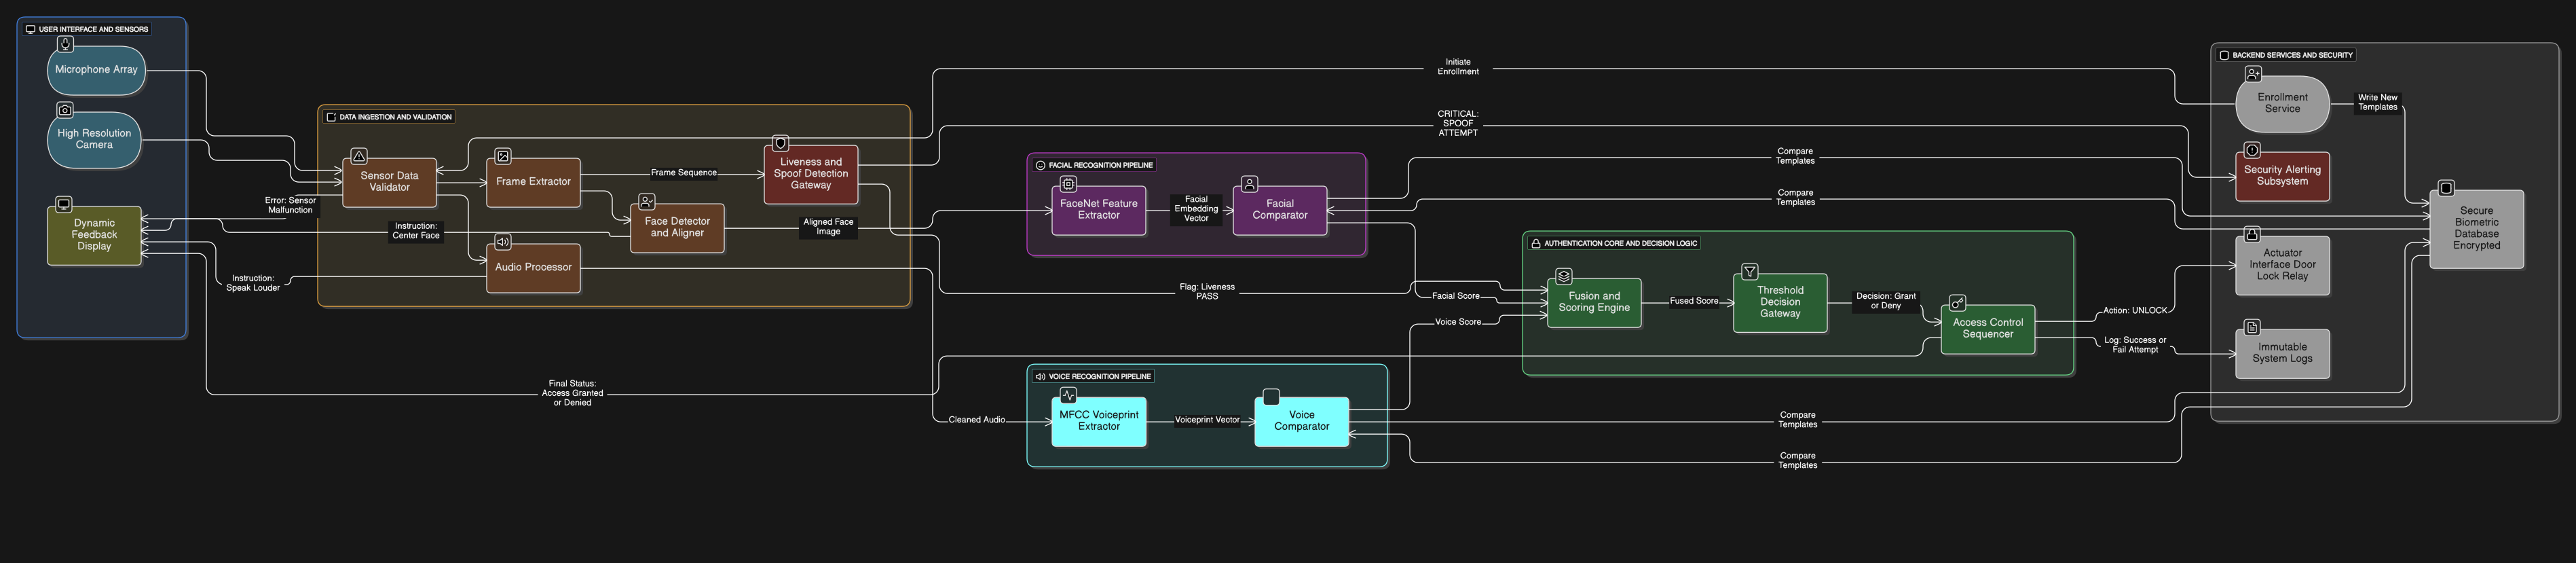
\includegraphics[width=\textwidth]{block_diagram.png}
    \caption{High-Level System Architecture Flow Chart}
    \label{fig:flowchart}
\end{figure}

% --- SECTION 4: REFERENCES ---
\section{References}
\begin{thebibliography}{9}

\bibitem{facenet}
Schroff, F., Kalenichenko, D., \& Philbin, J. (2015). FaceNet: A Unified Embedding for Face Recognition and Clustering. \textit{2015 IEEE Conference on Computer Vision and Pattern Recognition (CVPR)}.

\bibitem{arcface}
Deng, J., Guo, J., Xue, N., \& Zafeiriou, S. (2019). ArcFace: Additive Angular Margin Loss for Deep Face Recognition. \textit{2019 IEEE/CVF Conference on Computer Vision and Pattern Recognition (CVPR)}.

\bibitem{speechbrain}
Ravanelli, M., et al. (2021). SpeechBrain: A General-Purpose Speech Toolkit. \textit{arXiv preprint arXiv:2106.04624}.

\bibitem{ecapa}
Desplanques, B., Thienpondt, J., \& Demuynck, K. (2020). ECAPA-TDNN: Emphasized Channel Attention, Propagation and Aggregation in TDNN Based Speaker Verification. \textit{2020 IEEE International Conference on Acoustics, Speech and Signal Processing (ICASSP)}.

\bibitem{retinaface}
Chi, Jin, et al. (2020). RetinaFace: Single-Shot Multi-Level Face Localisation in the Wild. \textit{2020 IEEE/CVF Conference on Computer Vision and Pattern Recognition (CVPR)}.

\end{thebibliography}

\end{document}